\documentclass{article}

% Paquetes comunes
\usepackage[utf8]{inputenc}
\usepackage[T1]{fontenc}
\usepackage[spanish]{babel}
\usepackage{amsmath, amssymb}
\usepackage{graphicx}
\usepackage{float}
\usepackage{geometry}
\usepackage{hyperref}
\usepackage{fancyhdr}
\usepackage{textcomp}
\usepackage{circuitikz}
% Saltar entre párrafos - sin sangrías
\usepackage{parskip}

% Márgenes
\geometry{a4paper, margin=2.5cm}

% Encabezado y pie de página
\pagestyle{fancy}
\fancyhf{}
\fancyhead[L]{\textbf{Tarea 1} - Tomas Infante}
\fancyhead[R]{IEE2513}
\fancyfoot[C]{\thepage}

\title{Tarea 2}
\author{Tomas Infante}
\date{\today}
\begin{document}
\begin{figure}[H]
    \centering
    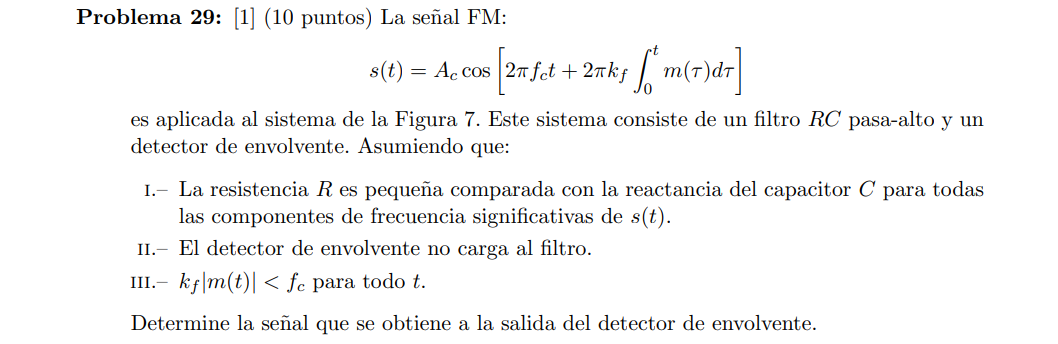
\includegraphics[width=1\textwidth]{Problema_29.png}
    \label{Problema_29}
\end{figure}
Para resolver este problema lo primero es entender que la asumicion I. nos dice que:
\[
R \ll \frac{1}{sC} \quad \longrightarrow \quad sRC \ll 1
\]
\begin{figure}[H]
    \centering
    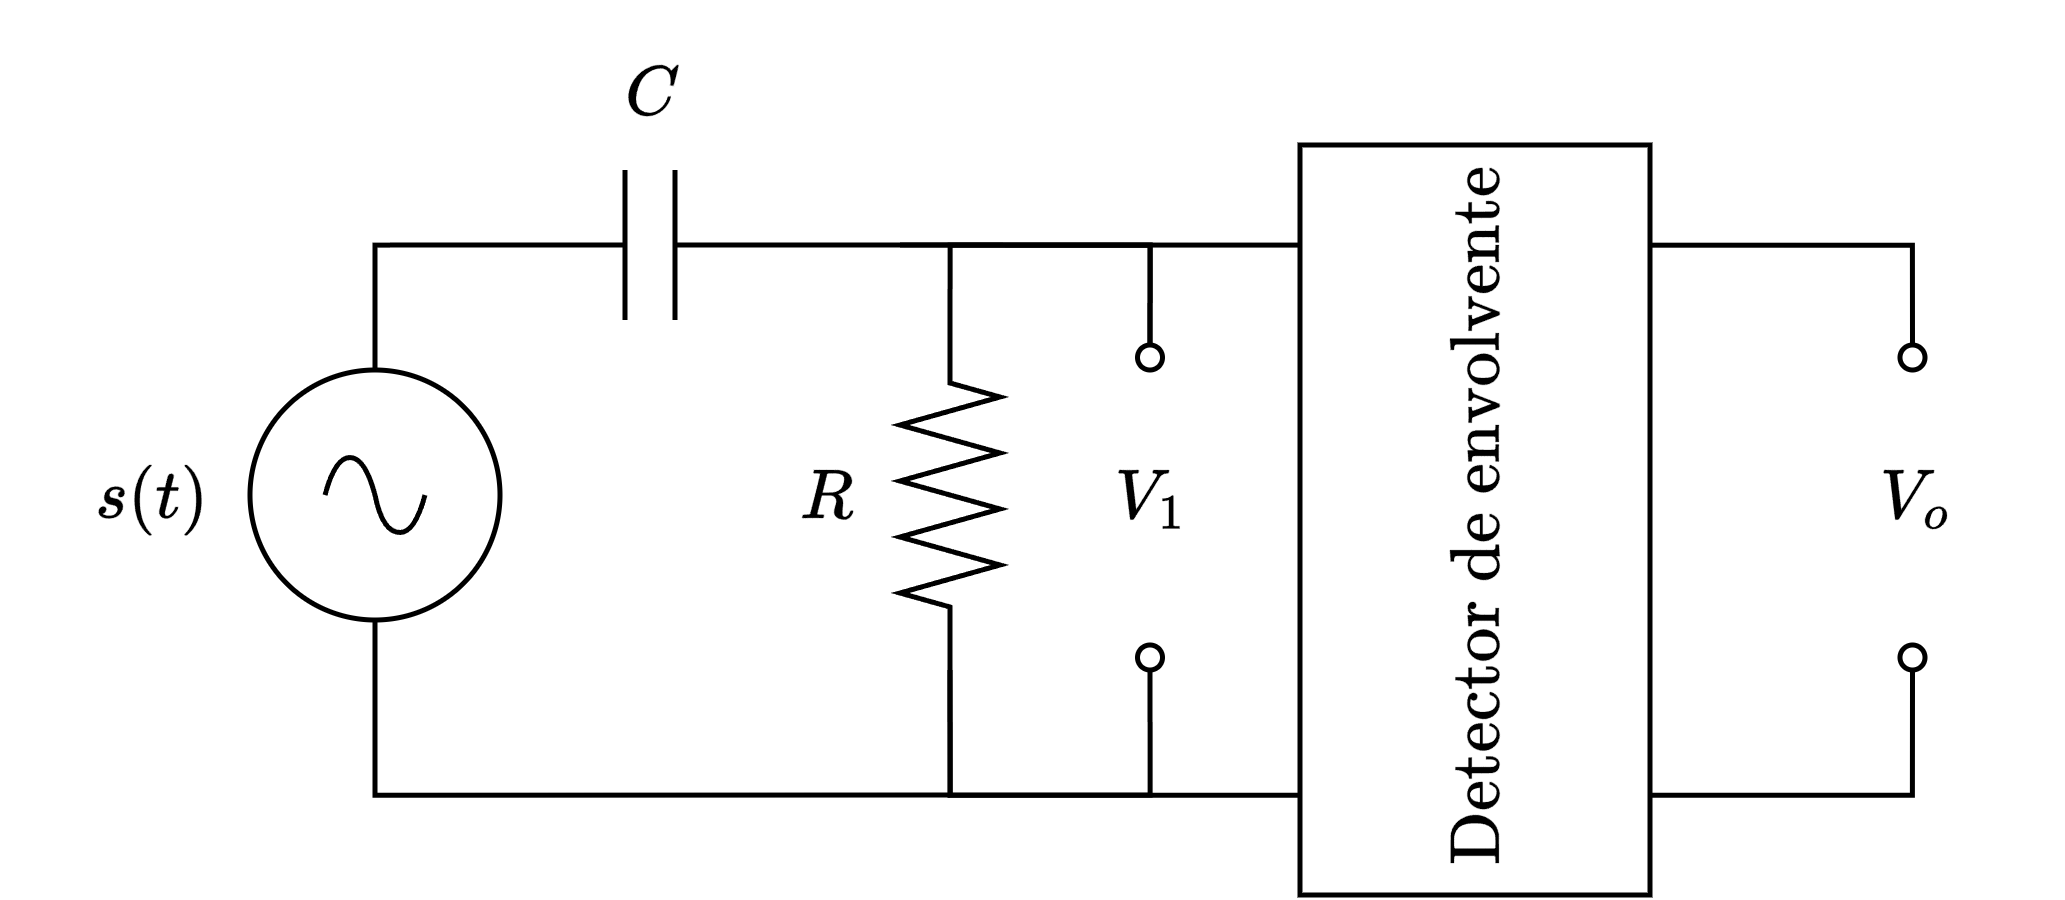
\includegraphics[width=0.6\textwidth]{Circuito_P29.png}
    \label{Circuito_P29}
\end{figure}
Del circuito anterior podemos encontrar una expresion para \(V_1\) en funcion de \(s(t)\) (Teniendo en cuenta que el detector no carga el filtro). Ya que es un divisor de voltaje:
\[
S(s)\frac{R}{1+\frac{1}{sC}} = V_1(s) \quad \longrightarrow \quad S(s)\frac{sRC}{1+sRC} = V_1(s) 
\]
Como \(sRC \ll 1\) la expresion final se puede aproximar muy fielmente a:
\[
S(s)\frac{sRC}{1} = V_1(s) \quad \longrightarrow \quad S(s)RC = V_1(s) 
\]
Nosotros sabemo que multiplicar por \(s\) en frecuencia es equivalente a derivar en el tiempo por lo que se sigue que:
\[
RC\frac{d}{dt}(s(t))= v_1(t)
\]
Derivamos \(s(t)\):
\[
\frac{d}{dt}(s(t))=-A_c\sin\left[2\pi f_c t+2\pi k_f\int_{0}^{t}m(\tau)d\tau\right](2\pi f_c +2\pi k_f m(t))
\]
Podemos definir:
\[
\sin\left[2\pi f_c t+2\pi k_f\int_{0}^{t}m(\tau)d\tau\right] = \sin(\phi(t))
\]
Sabamos simplemente que es una señal oscilante de alta frecuencia. En tal caso tenemos que:
\[
\frac{d}{dt}(s(t))=-A_c\sin(\phi(t))(2\pi f_c +2\pi k_f m(t))
\]
Factorizamos y reordenamos:
\[
\frac{d}{dt}(s(t))=-2\pi A_c(f_c + k_f m(t))\sin(\phi(t))
\]
Recordamos que:
\[
v_1(t) = RC\frac{d}{dt}(s(t))
\]
Reemplazamos
\[
v_1(t)=-2RC\pi RC A_c(f_c + k_f m(t))\sin(\phi(t))
\]
Esa es una modulacion AM, donde:
\[
A_m = -2RC\pi RC A_c
\]
Y como nos dicen que \(k_f|m(t)|<f_c\,\forall t\) no hay sobremodulacion. Y llegamos a:
\[
v_1(t)=A_m(f_c + k_f m(t))\sin(\phi(t))
\]
Como \(v_1(t)\) entra en el detector de envolvente, que vamos a asumir funciona correctamente, este va a detectar la envolvente de la señal de alta frecuancia es decir.
\[
v_o(t) = |A_m|(f_c + k_f m(t)) = 2\pi RC A_c  (f_c + k_f m(t))
\]
\(v_o(t)\) es la salida del detector de envolvente.

\begin{figure}[H]
    \centering
    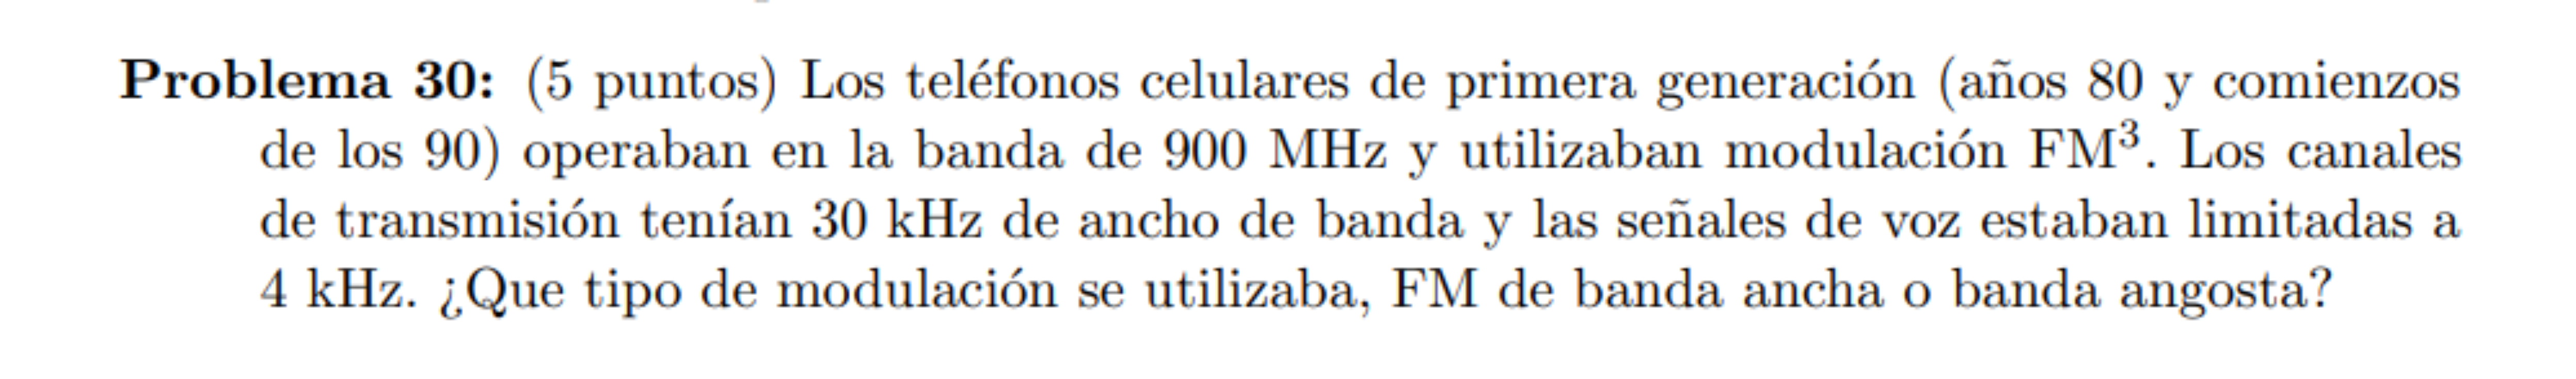
\includegraphics[width=1\textwidth]{Problema_30.png}
    \label{Problema_30}
\end{figure}
Debemos encontrar \(\beta\) y de esa manera poder saber si era banda ancha o banda angosta:
\[
\beta = \frac{\Delta f}{f_m}
\]
Y el ancho de banda segun la regal de carson se puede aproximar a:
\[
B \approx 2\left(\Delta f+f_m\right)
\]
Segun datos del enunciado tenemos que:
\[
B = 30\, \text{kHz} \quad f_m = 4\, \text{kHz}
\]
En tal caso:
\[
30\, \text{kHz} = 2 ( \Delta f + 4\, \text{kHz})
\]
Resolvemos para \(f_m\):
\[
\Delta f = \frac{30\, \text{kHz}}{2} -4\, \text{kHz} = 11\, \text{kHz}
\]
Por lo tanto:
\[
\beta = \frac{11\, \text{kHz}}{4\, \text{kHz}} = 2.75
\]
Y como \(2.75 > 0.3\). Podemos decir que esta modulado en banda ancha.
\begin{figure}[H]
    \centering
    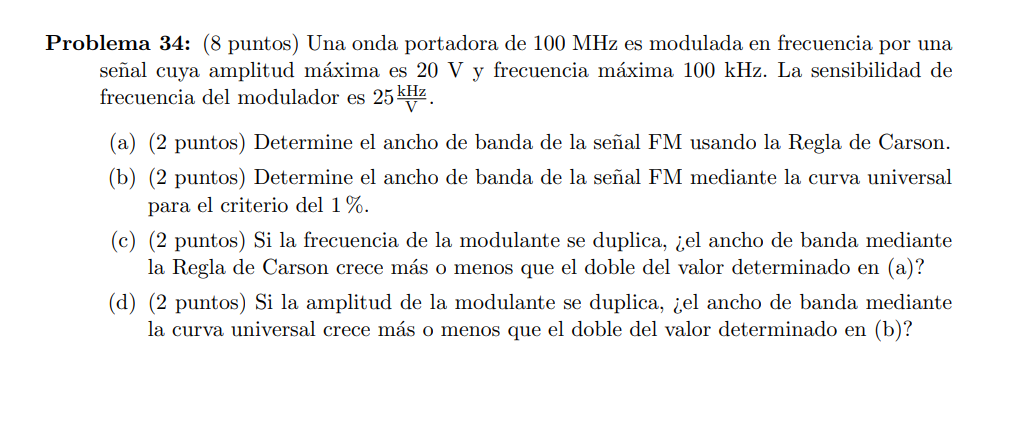
\includegraphics[width=1\textwidth]{Problema_34.png}
    \label{Problema_34}
\end{figure}
Primero calculamos \(\Delta f\) que es:
\[
\Delta f = k_f A_m \quad \longrightarrow \quad \Delta f = 25\,\frac{\text{kHz}}{\text{V}}20\,\text{V} = 500\, \text{kHz}
\]
\subsection*{a)}
De esta manera, el ancho de banda segun regla de Carson seria:
\[
B = 2(\Delta f +f_m) 
\]
\[
B = 2(500\, \text{kHz} +100\,\text{kHz}) = 1.2\,\text{MHz}
\]
\subsection*{b)}
Con el criterio del 1\% hay que calcular \(\beta\).
\[
\beta = \frac{\Delta f}{f_m} = \frac{500}{100}= 5
\]
Por lo tanto vamos a la grafica:
\begin{figure}[H]
    \centering
    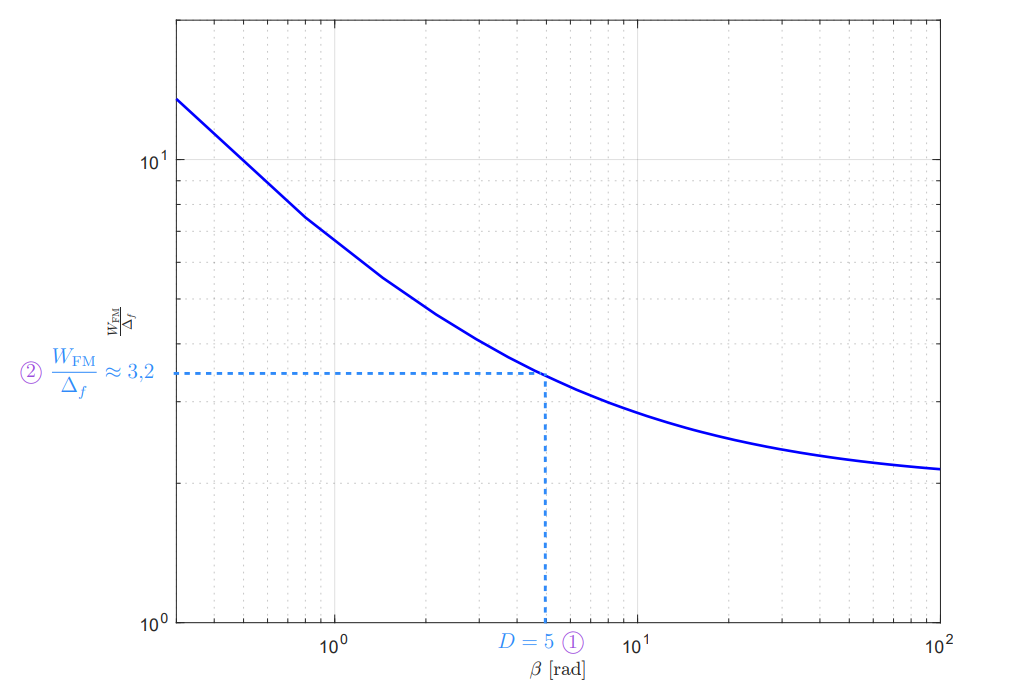
\includegraphics[width=0.7\textwidth]{Curva_Universal.png}
    \label{Curva_Universal}
\end{figure}
Donde obtenemos que:
\[
\frac{B}{\Delta f}=3.2 \quad \longrightarrow \quad B=3.2 \Delta f
\]
Por lo tanto:
\[
B = 3.2(500\,\text{kHz})=1.6\,\text{MHz}
\]
\subsection*{c)}
Si la amplitud de la modulante se duplica, entonces tenemos que, como:
\[
\Delta f \propto A_m \quad \longrightarrow \quad \Delta f' = 2\Delta f
\]
Entonces si usamos la regla de Carson:
\[
B' = 2(\Delta f'+f_m)
\]
Que es equivalente a:
\[
B' = 2(2\Delta f+f_m) = 2(\Delta f + \Delta f+f_m) = 2(\Delta f+f_m) + 2\Delta f
\]
Por lo tanto:
\[
B' = B + 2\Delta f
\]
Es decir, crece a menos que el doble  que a) ya que:
\[
2\Delta f < 2(\Delta f + f_m)
\]
Para ser precisos:
\[
B' = 1.2\,\text{MHz} + 2 (500\,\text{kHz}) = 2.2\,\text{MHz}
\]
\subsection*{d)}
Nuevamente al igual que antes:
\[
\Delta f \propto A_m \quad \longrightarrow \quad \Delta f' = 2\Delta f
\]
En tal caso \(\beta'\):
\[
\beta' = \frac{\Delta f'}{f_m}
\]
Operamos:
\[
\beta' = \frac{2\Delta f}{f_m} = 2\frac{\Delta f}{f_m} = 2\beta
\]
Entonces:
\[
\beta' = 2(5) = 10
\]
Vamos a la curva universal y vemos que para ese valor de \(\beta\) tenemos que:
\begin{figure}[H]
    \centering
    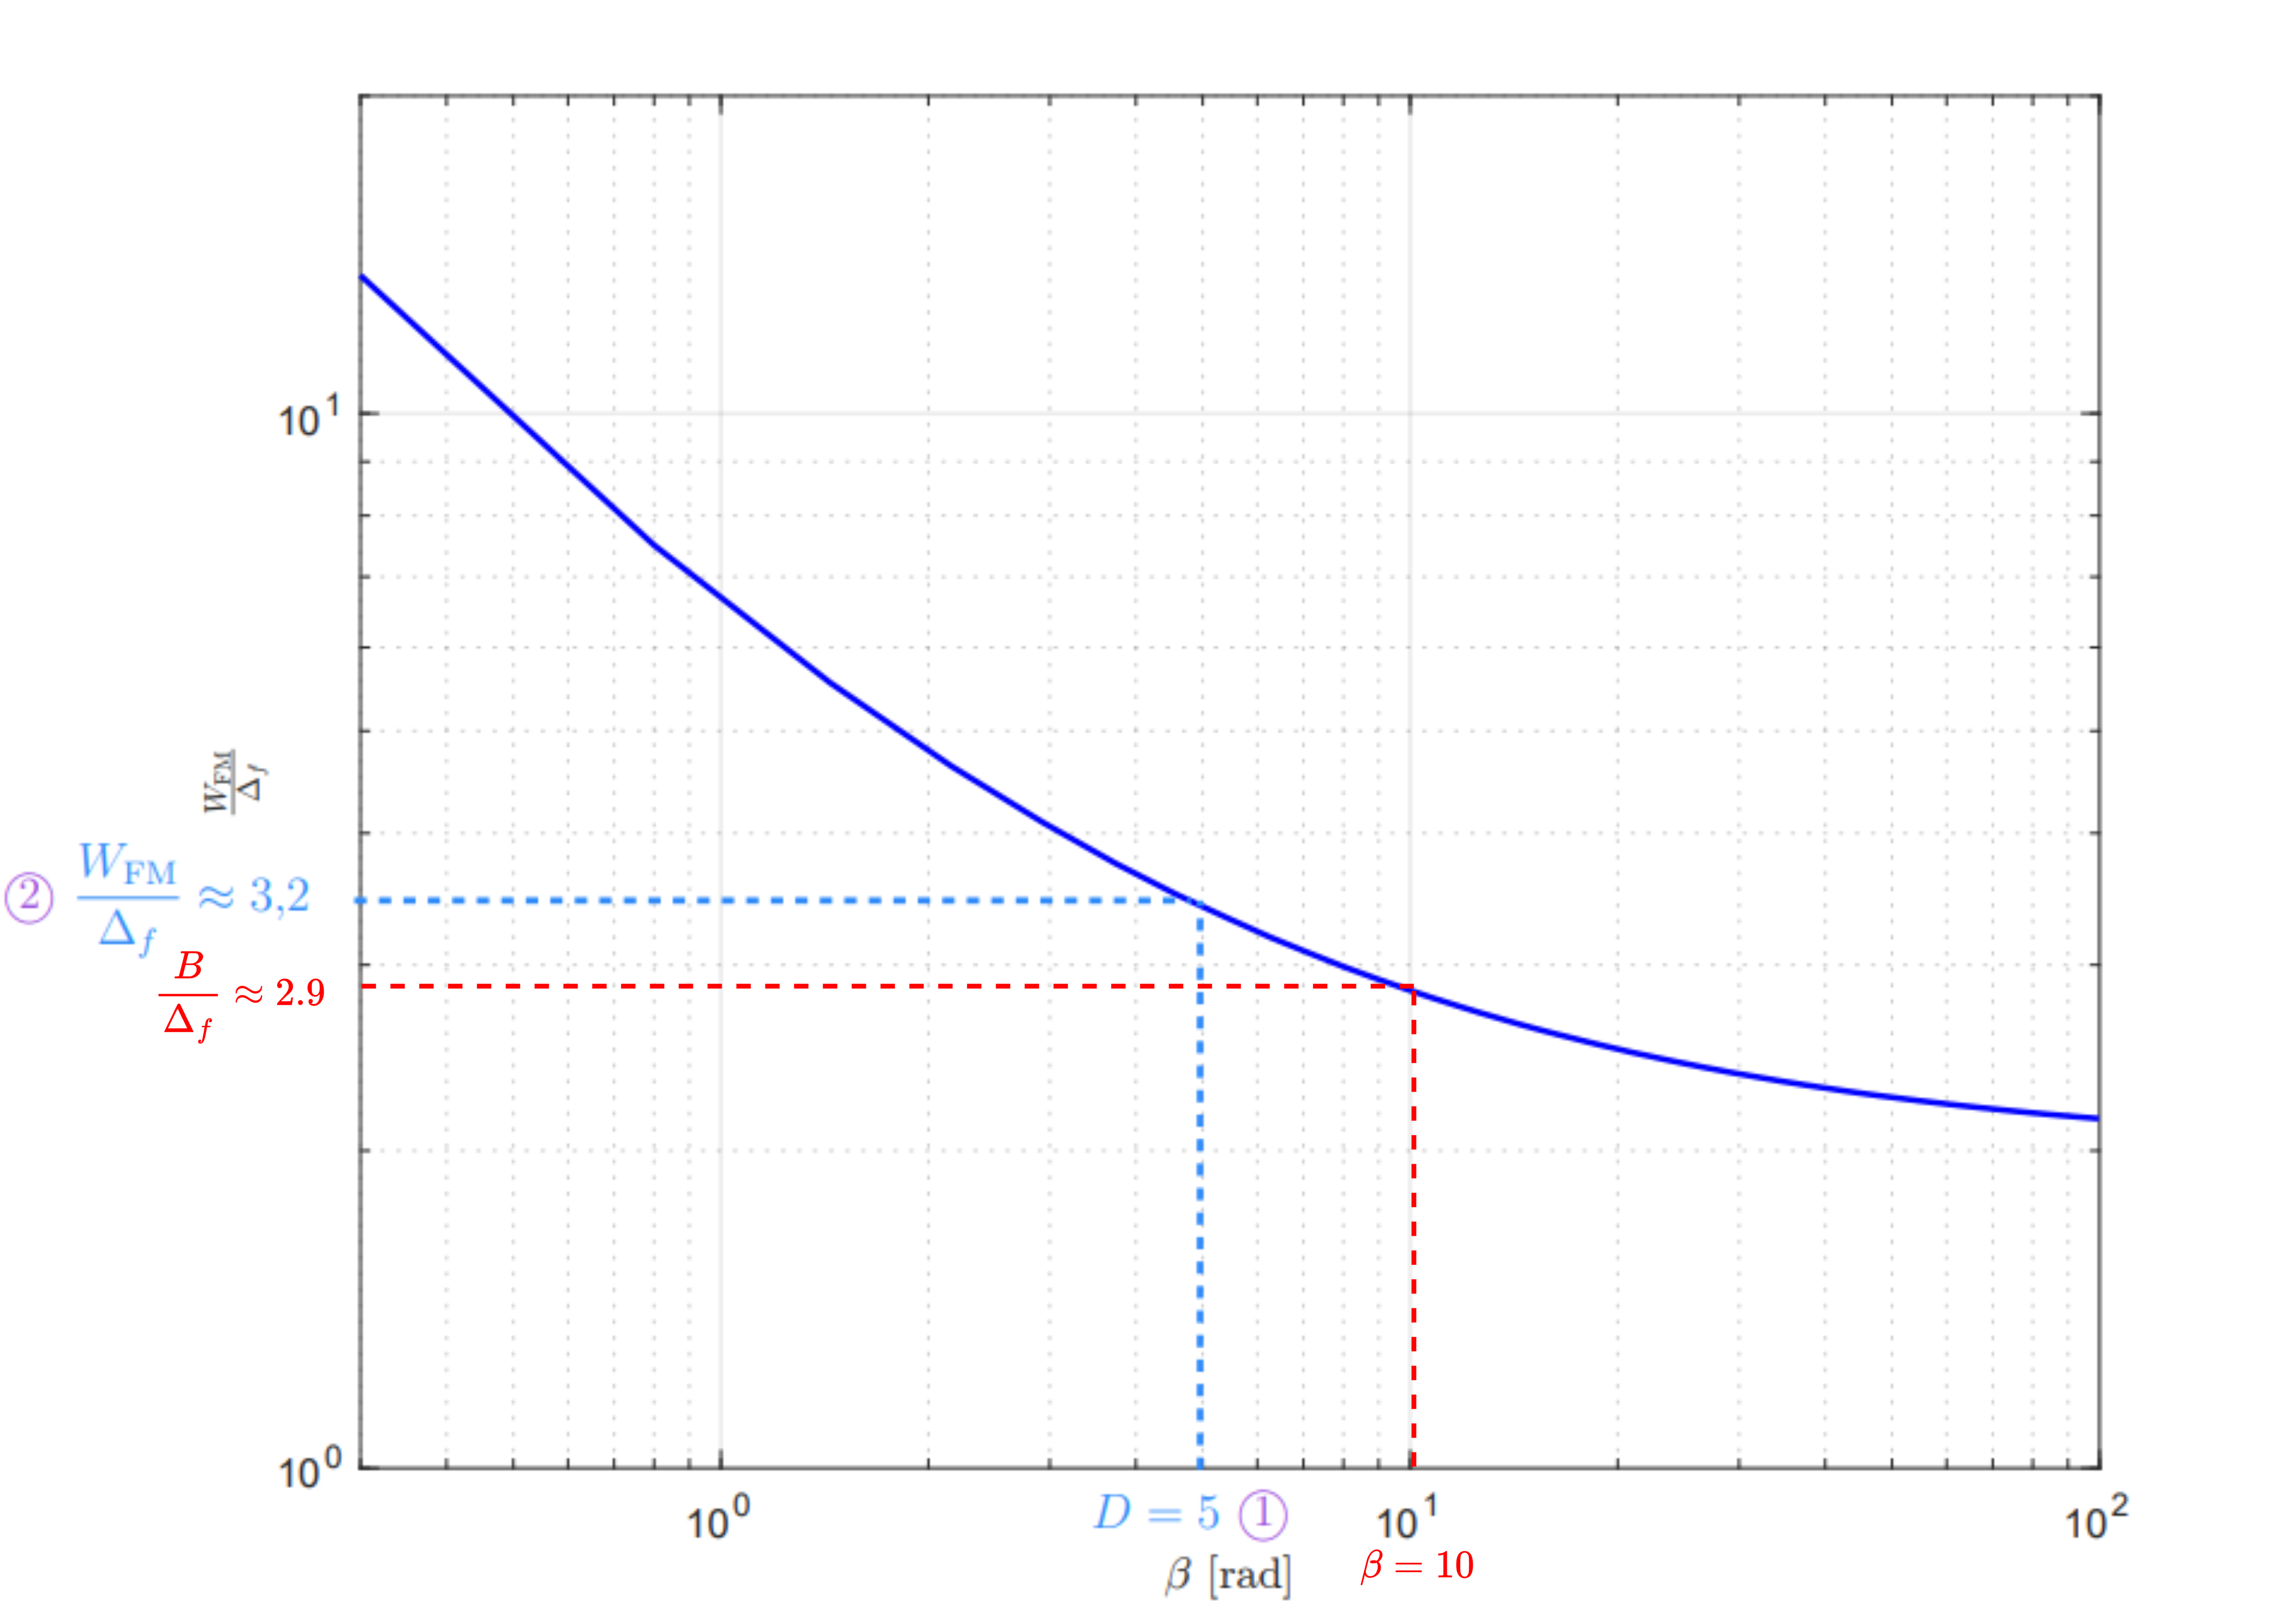
\includegraphics[width=0.7\textwidth]{Curva_Universal_2.png}
    \label{Curva_Universal_2}
\end{figure}
Donde obtenemos que:
\[
\frac{B'}{\Delta f'}=2.9 \quad \longrightarrow \quad B'=2.9 \Delta f'
\]
Por lo tanto:
\[
B'=2.9 (2\Delta f) = 2.9(2(500\,\text{kHz})) = 2.9\, \text{MHz}
\]
Osea tambien el ancho de banda es menor que el doble que el obtenido en b).
\begin{figure}[H]
    \centering
    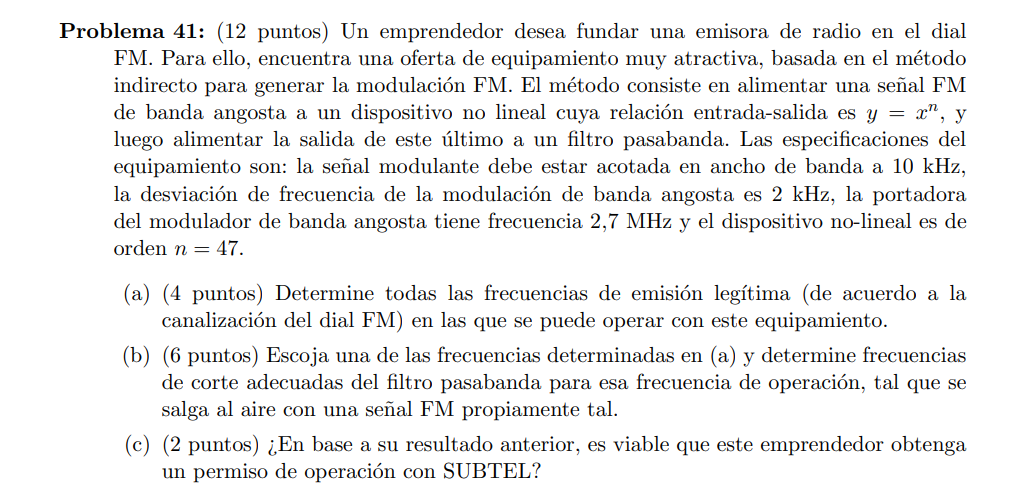
\includegraphics[width=1\textwidth]{Problema_41.png}
    \label{Problema_41}
\end{figure}
\begin{figure}[H]
    \centering
    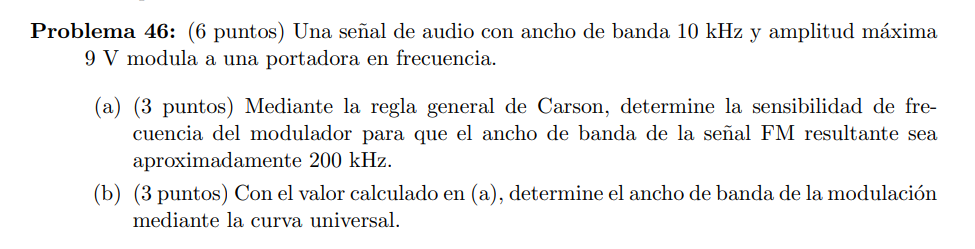
\includegraphics[width=1\textwidth]{Problema_46.png}
    \label{Problema_46}
\end{figure}
\subsection*{a)}
La regla de Carson nos dice que:
\[
B = 2(\Delta f +f_m) 
\]
Y si recordamos que \(\Delta f = k_f A_m\) tenemos que la regla de Carson se puede reescribir como:
\[
B = 2(k_f A_m +f_m) 
\]
Despejamos la sensibilidad de frecuencia del modulador:
\[
B = 2(k_f A_m +f_m) \quad \longrightarrow \quad \frac{\frac{B}{2} - f_m}{A_m} = k_f
\]
Reemplazamos:
\[
k_f = \frac{\frac{200\,\text{kHz}}{2}-10\,\text{kHz}}{9\,\text{V}} = 10 \,\frac{\text{kHz}}{\text{V}}
\]
\subsection*{b)}
De manera similar, para usar la curva universal hay que calcular \(\beta\):
\[
\beta =\frac{\Delta f}{f_m}
\]
Donde:
\[
\Delta f = 10 \,\frac{\text{kHz}}{\text{V}} \cdot 9\,\text{V}=90\,\text{kHz}
\]
Por lo tanto:
\[
\beta =\frac{90}{10} = 9
\]
No vamos a la curva universal y notamos que para ese valor de \(\beta\) tenemos:
\[
\frac{B}{\Delta f}\approx 2.9 \quad \longrightarrow \quad B = 2.9 \Delta f 
\]
\[
B = 2.9 \cdot 90\,\text{kHz}= 261\,\text{kHz}
\]
\end{document}